\documentclass[class=minimal, border = 0pt, crop]{standalone}
\usepackage{pgf}
\usepackage{tikz}
\usepackage[utf8]{inputenc}
\usetikzlibrary{arrows,automata,shapes,calc, backgrounds}
\usetikzlibrary{positioning}
\pagestyle{empty}
\newcommand\irregularcircle[2]{% radius, irregularity
  \pgfextra {\pgfmathsetmacro\len{(#1)+rand*(#2)}}
  +(0:\len pt)
  \foreach \a in {10,20,...,350}{
    \pgfextra {\pgfmathsetmacro\len{(#1)+rand*(#2)}}
    -- +(\a:\len pt)
  } -- cycle
}
\tikzset{
    %Define standard arrow tip
    >=stealth',
    % Define arrow style
    pil/.style={
           ->,
           red,
           },
    pilar/.style={
           ->,
           blue,
}
}
\begin{document}
\centering
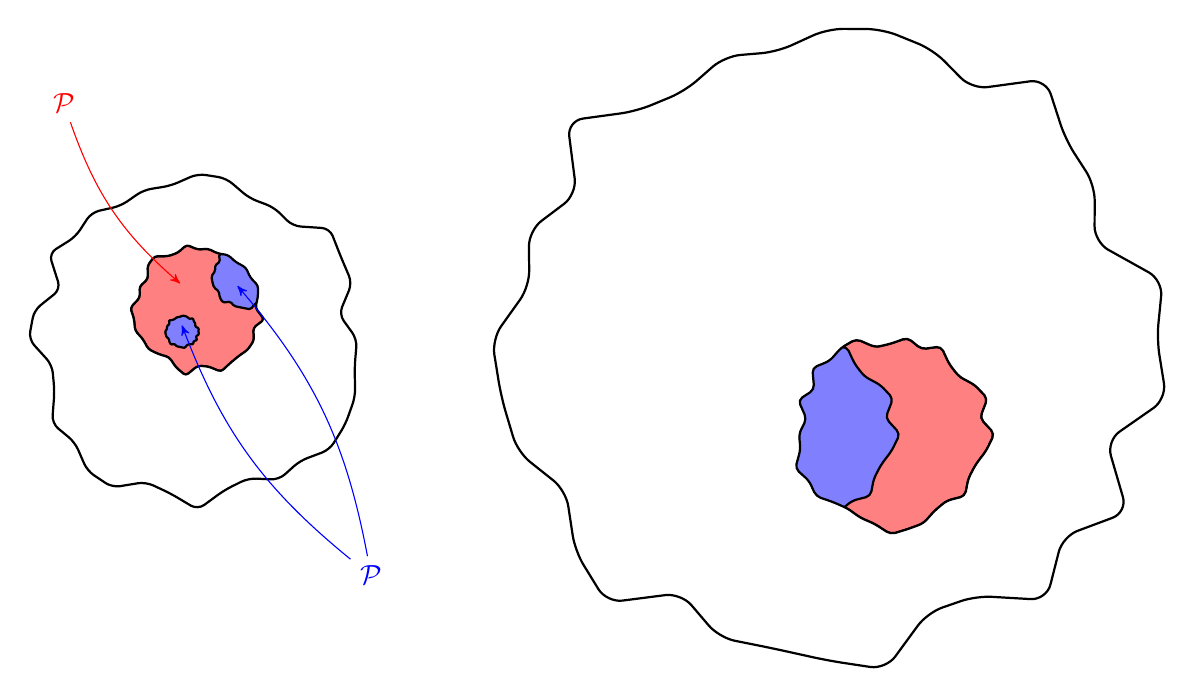
\begin{tikzpicture}
  	\coordinate (o) at (0,0) {};
  	\coordinate (p) at (-8,0);
  	\coordinate (q) at (0.8,-1.2);
  	\coordinate (r) at (-8,0.4);
  	\pgfmathsetseed{1990}\draw[rounded corners=2mm,thick] (o) \irregularcircle{4cm}{4mm};
  	\pgfmathsetseed{2001}\draw[rounded corners=1mm, thick] (p) \irregularcircle{2cm}{2mm};
  	\begin{scope}
  		\pgfmathsetseed{2008}\draw[clip] (q) [rounded corners=0.6mm] \irregularcircle{1.2cm}{1.2mm};
  		\pgfmathsetseed{2008}\draw[rounded corners=0.6mm,thick,fill=red!50] (q) \irregularcircle{1.2cm}{1.2mm};
  		\pgfmathsetseed{2008}\draw[rounded corners=0.6mm,thick,fill=blue!50] (-0.4,-1.2) \irregularcircle{1.2cm}{1.2mm};
	\end{scope}
	\pgfmathsetseed{2008}\draw[rounded corners=0.6mm,thick] (q) \irregularcircle{1.2cm}{1.2mm};
	\begin{scope}
	\pgfmathsetseed{2014}\draw[clip] (r) [rounded corners=0.4mm] \irregularcircle{0.8cm}{0.8mm};
	\pgfmathsetseed{2014}\draw[rounded corners=0.4mm,thick,fill=red!50] (r) \irregularcircle{0.8cm}{0.8mm};
	\pgfmathsetseed{1990}\draw[rounded corners=0.1mm,thick,fill=blue!50] (-8.2,0.1) \irregularcircle{0.2cm}{0.2mm};
	\pgfmathsetseed{1990}\draw[rounded corners=0.2mm,thick,fill=blue!50] (-7.4,0.8) \irregularcircle{0.4cm}{0.4mm};
	\end{scope}
 	\pgfmathsetseed{2014}\draw[rounded corners=0.4mm,thick] (r) \irregularcircle{0.8cm}{0.8mm};
  	\node (a) at (-8.25,0.3) [] {};
  	\node (b) at (-7.6,0.8) [] {};
  	\node (c) at (-8.1,0.6) [] {};
  	\node (d) at (-5.8,-3) [] {$\color{blue}\mathcal{P}$};
  	\node (e) at (-9.7,3) [] {$\color{red}\mathcal{P}$};
%  	\node (c) at (0,4) [label=above:$\mathcal{S}$] {};
%  	\node (d) at (-8,2) [label=above:$\mathcal{P}$] {};
%  	\draw [pil] (q.south west) to [bend left=45] node [] {} (r.south east); 
  	\draw [pilar] (d) to [bend left=15] node [] {} (a);
  	\draw [pilar] (d) to [bend right=15] node [] {} (b);
  	\draw [pil] (e) to [bend right=15] node [] {} (c);
\end{tikzpicture}
\end{document}